
\documentclass[12pt, a4paper]{article}

\usepackage[utf8]{inputenc}
\usepackage[T1]{fontenc}
\usepackage[russian]{babel}
\usepackage[oglav,spisok,boldsect,eqwhole,figwhole,hyperref,hyperprint,remarks,greekit]{./style/fn2kursstyle}
\graphicspath{{./style/}{./figures/}}

\usepackage{multirow}
\usepackage{supertabular}
\usepackage{multicol}
\usepackage{amsmath}
\usepackage{afterpage}
% Параметры титульного листа
\title{Раскрытие статической неопределимости балки при
	поперечном изгибе \\ Вариант 15}
\author{В.\,Г.~Пиневич}
\supervisor{Е.\,А.~Максимова}
\group{ФН2-71Б}
\date{2023}

% Переопределение команды \vec, чтобы векторы печатались полужирным курсивом
\renewcommand{\vec}[1]{\text{\mathversion{bold}${#1}$}}%{\bi{#1}}
\newcommand\thh[1]{\text{\mathversion{bold}${#1}$}}
%Переопределение команды нумерации перечней: точки заменяются на скобки
\renewcommand{\labelenumi}{\theenumi)}
\begin{document}
	
	\maketitle
	
	\tableofcontents
	
	\newpage
	\section-{Обозначения}
	
	\vspace{-0.5em}
	
	$L$ --- длина трети балки, м;
	
	$b$ --- основание прямоугольного поперечного сечения балки, м;
	
	$h$ --- высота прямоугольного поперечного сечения балки, м;
	
	$E$ --- продольный модуль упругости (модуль Юнга), Па;
	
	$J_3$ --- осевой момент инерции относительно нейтральной оси, $\text{м}^4$;
	
	$W_3$ --- момент сопротивления сечения при изгибе, $\text{м}^3$;
	
	$R_3$ --- сила реакции, приложенная вместо отброшеной связи, Н;
	
	$M_i$ --- момент, Н$\cdot$м;
	
	$P_i$ --- сила или реакция, Н;
	
	$q^{\circ}$ --- равномерно распределённая нагрузка, Н/м;
	
	$M_3$ --- изгибающий момент, Н$\cdot$м;
	
	$Q$ --- перерезывающая сила, Н;
	
	$w$ --- величина прогиба балки, м; 
	
	$\sigma_{11}^{max}$ --- максимальное растягивающее напряжение, Па.
	
	\newpage
	
	\section{Постановка задачи}
	
	\begin{figure}[!h]
		\centering
		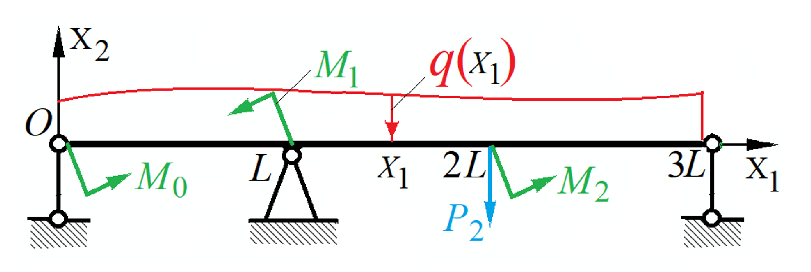
\includegraphics[width=0.75\linewidth]{plot-1}
		\caption{Общая схема нагружения статически неопределимой балки}
		\label{start-pic-1}
	\end{figure}
	
	В соответствии с индивидуальным заданием необходимо использовать тип связи $R_3$. Это означает, что при раскрытии статической неопределимости шарнирную опору балки при $x_1 = 3L$ следует заменить подлежащей определению реакцией $R_3$ с положительным направлением вдоль положительного направления координатной оси $Ox_2$. Положительные направления нагружающих силовых факторов соответствуют их направлениям, отмеченным на рис.~\ref{start-pic-1} стрелками. 
	
	Для индивидуального варианта заданы моменты $M_0 = M$, $M_1 = -M$, $M_2 = 0$, прикладываемая сила $P_2 = -P$ и распределённая нагрузка $q(x_1) = q^{\circ}$, $x_1 \in (0, 2L)$. 
	
	При этом $M = 2000 \ \text{Н} \! \cdot \! \text{м}$, $P = 1000$ Н, $q^{\circ} = 1000$ Н/м, $L = 1$ м. Прямоугольное поперечное сечение балки имеет основание $b = 30$ мм и высоту $h = 65$ мм. Балка выполнена из малоуглеродистой стали с продольным модулем упругости (модулем Юнга) $E = 210$ ГПа.
	
	\newpage
	
	\section{Схема нагружения в соответствии с индивидуальным заданием}
	
	\vspace{-1em}
	
	\begin{figure}[!h]
		\centering
		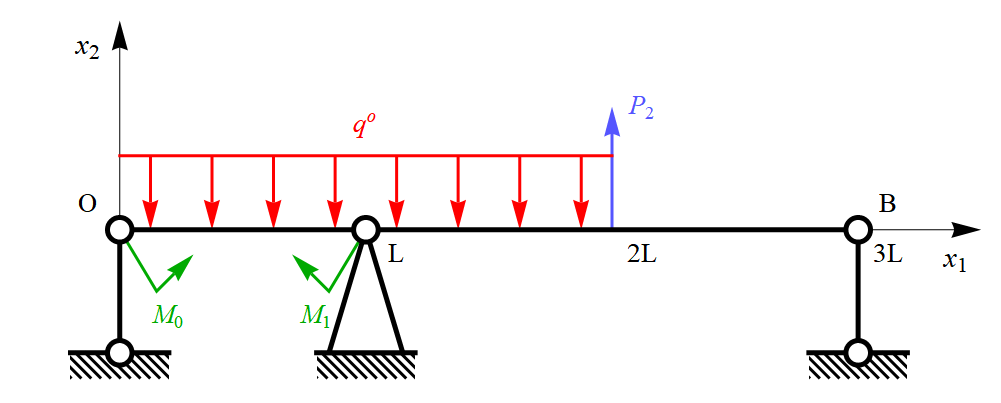
\includegraphics[width=0.75\linewidth]{plot-2}
		\caption{Схема нагружения балки для заданного варианта}
	\end{figure}
	
	\section{Степень статической неопределимости балки}
	
	Для полученной системы неизвестными являются 3 реакции в шарнирах. Однако можем записать всего 2 уравнения равновесия, а именно уравнение равновесия сил в проекции на вертикальную ось и уравнение равновесия моментов относительно точки. Значит, система является 1 раз статически неопределимой, то есть для определения всех возникающих реакций недостаточно только уравнений статики.
	
	\section{Переход к статически определимой балке}
	
	В соответствии с индивидуальным вариантом отбросим указанную в задании наложенную связь $P_3$ и заменим её соответствующей реакцией $R_3$. Таким образом осуществим переход к статически определимой балке.
	
	\begin{figure}[!h]
		\centering
		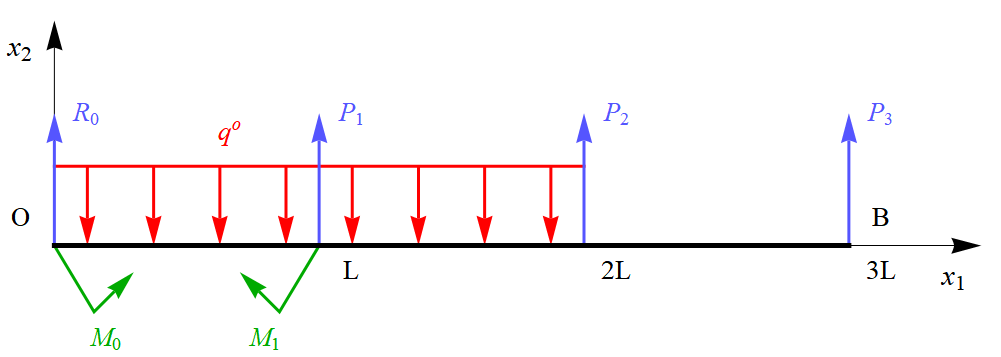
\includegraphics[width=0.75\linewidth]{plot-3}
		\caption{Нагружение для статически определимой балки}
	\end{figure}
	
	\newpage
	
	Уравнение равновесия сил в проекции на вертикальную ось $Ox_2$ имеет вид
	\begin{equation*}
		\sum P = 0 \ \Rightarrow \ R_3 + P_1 + P_2 + P_0 - 2L \cdot q^{\circ} = 0.
	\end{equation*}
	
	Аналогично уравнение равновесия моментов относительно точки $B$
	\begin{equation*}
		\sum M = 0 \ \Rightarrow \ M_0 - M_1 + 2 L \cdot P_1 + L \cdot P_2 + 3 L \cdot P_0 - L^2 \cdot q^{\circ} = 0.
	\end{equation*}
	
	Откуда получим
	\begin{equation}
		\begin{cases} \vspace{0.75em}
			P_1 = \dfrac{1}{L} \left( M_0 - M_1 \right) - 3 R_3 - 2 P_2 + 5 L \cdot q^{\circ}, \\ 
			P_0 = \dfrac{1}{L} \left( M_1 - M_0 \right) + 2 R_3 + P_2 - 3 L \cdot q^{\circ}. \\
		\end{cases}
		\label{eqP0P1}
	\end{equation}
	
	\section{Балка под действием только реакции $R_3$}
	
	Будем считать, что на балку действует только реакция $R_3$, приложенная вместо отброшенной связи, а все остальные нагружающие силовые факторы отсутствуют.
	
	\begin{figure}[!h]
		\centering
		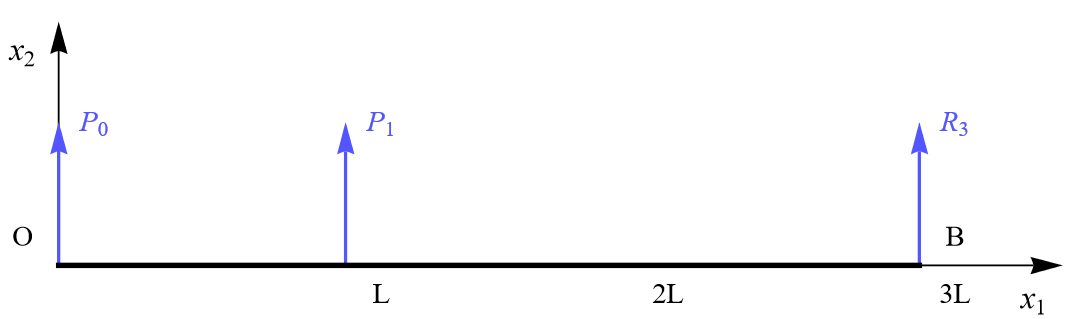
\includegraphics[width=0.75\linewidth]{plot-4}
		\caption{Нагружение балки только реакцией $R_3$}
	\end{figure}
	
	Уравнения равновесия сил в проекции на вертикальную ось $Ox_2$ и моментов относительно точки $B$ в этом случае имеют вид
	\vspace{-0.5em}
	\begin{equation*}
		\begin{cases}
			R_3 + P_1 + P_0 = 0, \\ 
			2L \cdot P_1 + 3L \cdot P_0 = 0. \\
		\end{cases}
	\end{equation*}
	
	Откуда получим
	\begin{equation}
		\begin{cases} \vspace{0.25em}
			P_1 = - 3 R_3, \\ 
			P_0 = 2 R_3. \\
		\end{cases}
		\label{eqP0P1R}
	\end{equation}
	
	Для упрощения выкладок введём функции
	\[
	f_n(x) = 
	\begin{cases}
		\dfrac{x^n}{n!}, & x > 0, \\ 
		0, & x \leq 0, \\
	\end{cases}
	\quad n \in \mathbb{Z}_+.
	\]
	
	\newpage
	
	Эти функции для $a \geq 0$ обладают свойствами:
	\begin{enumerate}
		\item $f_n'(x - a) = f_{n-1}(x - a)$ для $n \in \mathbb{N}$, причём $f_0'(x - a) = 0$.
		
		\vspace{0.25em}
		
		\item $\int\limits_0^{x} f_n(\xi - a) \, d \xi = f_{n+1}(x - a)$ для $n \in \mathbb{Z}_+$.
	\end{enumerate}
	
	Тогда можно записать выражение для изгибающего момента
	\[
	M_(x_1) = R_3 f_1(x_1 - 3L) + P_1 f_1(x_1 - L).
	\]
	
	Перерезывающая сила связана с изгибающим моментом следующим образом:
	\begin{equation}
		Q(x_1) = \dfrac{\mathrm{d} M_3(x_1)}{\mathrm{d} x_1}.
		\label{eqQ}
	\end{equation}
	
	Тогда
	\[
	Q(x_1) = R_3 f_0(x_1 - 3L) + P_1 f_0(x_1 - L).
	\]
	
	С учётом \eqref{eqP0P1R} имеем
	\begin{equation}
		\begin{cases} \vspace{0.25em}
			M_3(x_1) = R_3 \left( f_1\left(x_1\right) - 3 f_1\left(x_1 - L\right) \right), \\
			Q(x_1) = R_3 \left( f_0(x_1) - 3 f_0(x_1 - L) \right). \\
		\end{cases}
		\label{eqM3QR}
	\end{equation}
	
	Построим в безразмерных переменных эпюры изгибающего момента и перерезывающей силы в случае, когда действует только сила реакции $R_3$, приложенная вместо отброшенной связи.
	
	\begin{figure}[!h]
		\centering
		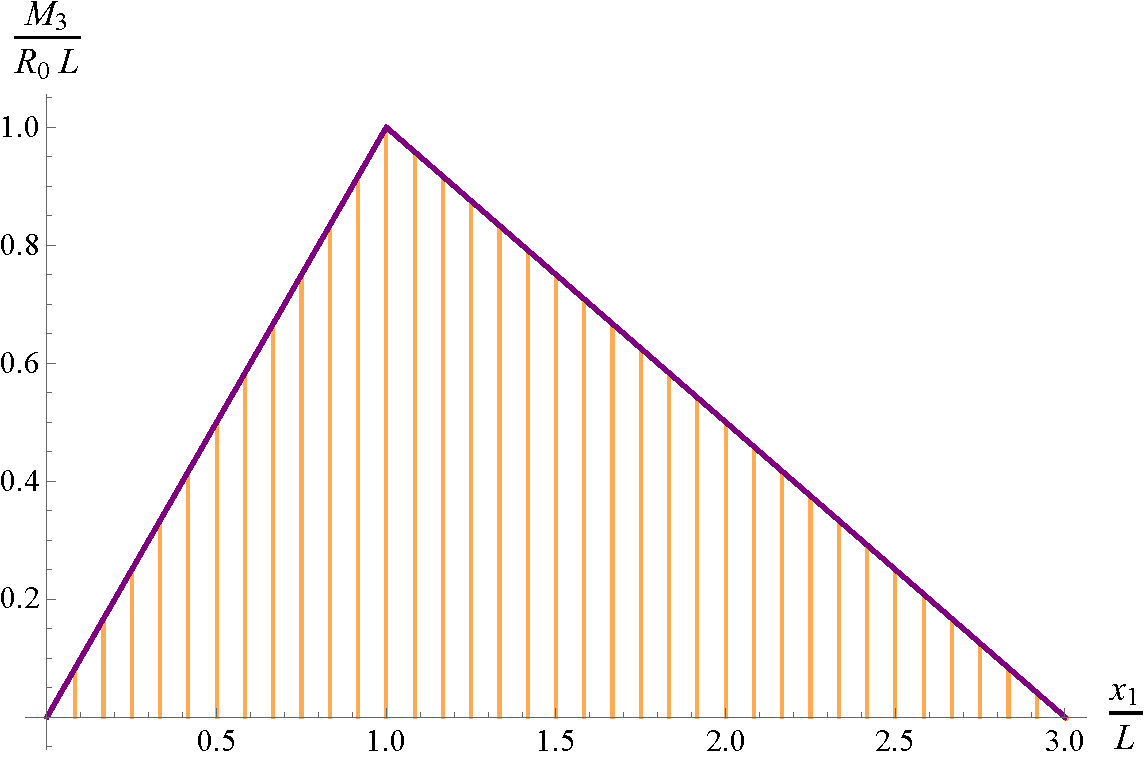
\includegraphics[width=0.75\linewidth]{plot-5}
		\caption{Эпюра изгибающего момента при действии только $R_3$}
	\end{figure} 
	
	\newpage
	
	\begin{figure}[!h]
		\centering
		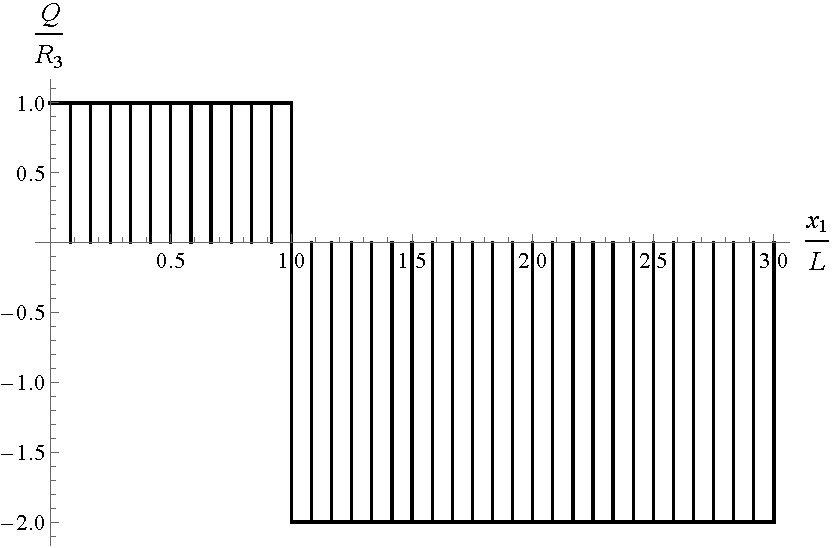
\includegraphics[width=0.75\linewidth]{plot-6}
		\caption{Эпюра перерезывающей силы при действии только $R_3$}
	\end{figure}
	
	\section{Прогиб балки только при реакции $R_3$} 
	
	Дифференциальное уравнение для прогиба балки
	\[
	\dfrac{\mathrm{d}^2 w(x_1)}{\mathrm{d} x_1^2} = \dfrac{M_3(x_1)}{E J_3}.
	\]
	
	Общее решение имеет вид
	\vspace{-0.5em}
	\begin{equation}
		w(x_1) = w(0) + w'(0) x_1 + \int\limits_0^{x_1} \! dt \int\limits_0^t \dfrac{M_3(\xi)}{E J_3} \, d \xi.
		\label{eqw}
	\end{equation}
	
	Ранее была отброшена одна связь в точке $x_1 = 3L$. Тогда остаётся 2 закрепления в точках $x_1 = L$ и $x_1 = 0$, в которых балка не должна прогибаться. В этом случае имеем следующие граничные условия:
	\vspace{-0.5em}
	\begin{equation}
		w(L) = 0, \quad w(0) = 0.
		\label{eqwGU}
	\end{equation}
	
	\vspace{-0.5em}
	
	С учётом \eqref{eqM3QR} прогиб балки под действием только реакции $R_3$
	\begin{equation}
		w(x_1) = \dfrac{R_3}{E J_3} \left( f_3(x_1) - 3 f_3(x_1 - L) + L^3 - \dfrac{1}{6} L^2 x_1 \right).
		\label{eqwR}
	\end{equation}
	
	В точке $x_1 = 0$
	\begin{equation}
		w_{R_3} = w(0) = \dfrac{L^3}{3 E J_3} R_3.
		\label{eqwR3}
	\end{equation}
	
	\newpage
	
	\section{Статически определимая балка без реакции $R_3$} 
	
	Будем считать, что на балку действуют все силовые факторы, кроме реакции $R_3$, приложенной вместо отброшенной связи.
	
	\begin{figure}[!h]
		\centering
		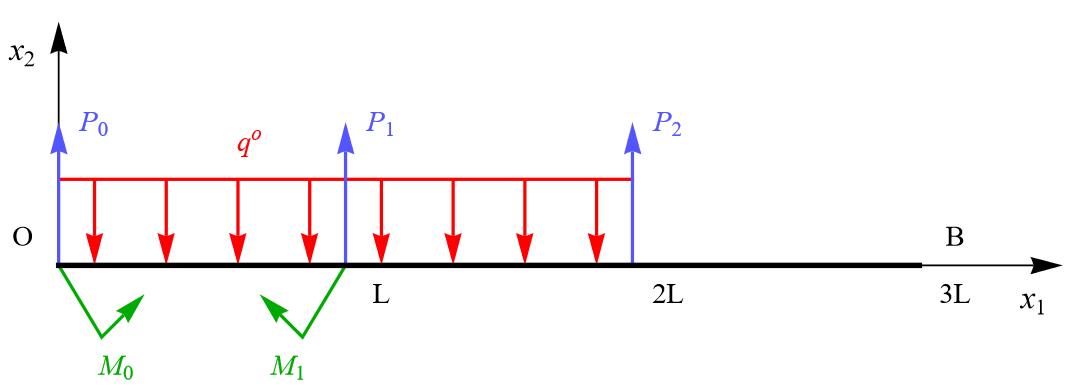
\includegraphics[width=0.75\linewidth]{plot-7}
		\caption{Нагружение балки без учёта реакции $R_3$}
	\end{figure}
	
	Уравнения равновесия сил в проекции на вертикальную ось $Ox_2$ и моментов относительно точки $O$ в этом случае имеют вид
	\vspace{-0.5em}
	\begin{equation*}
		\begin{cases}
			P_1 + P_2 + P_0 - 2L \cdot q^{\circ} = 0, \\
			M_0 - M_1 + L \cdot P_1 + 2L \cdot P_2 - 2 L^2 \cdot q^{\circ} = 0. \\
		\end{cases}
	\end{equation*}
	
	Откуда получим
	\begin{equation}
		\begin{cases} \vspace{0.75em}
			P_1 = \dfrac{1}{L} \left( M_1 - M_0 \right) - 2 P_2 + 2L \cdot q^{\circ}, \\ 
			P_0 = \dfrac{1}{L} \left( M_0 - M_1 \right) + P_2. \\
		\end{cases}
		\label{eqP0P1NOR}
	\end{equation}
	
	В этом случае выражение для изгибающего момента имеет вид
	\begin{equation}
		\begin{split}
			M_3(x_1) = M_1 f_0(x_1 - L) - M_0 f_0(x_1) & + P_1 f_1(x_1 - L) + \\ & + P_2 f_1(x_1 - 2L) - q^{\circ} f_2(x_1) + q^{\circ} f_2(x_1 - 2L).
		\end{split}
		\label{eqM3NOR}
	\end{equation}
	
	С учётом \eqref{eqQ} перерезывающая сила
	\begin{equation}
		Q(x_1) = P_1 f_0(x_1 - L) + P_2 f_0(x_1 - 2L) - q^{\circ} f_1(x_1) + q^{\circ} f_1(x_1 - 2L).\\
		\label{eqQNOR}
	\end{equation}
	
	Построим эпюры изгибающего момента и перерезывающей силы для статически определимой балки в случае, когда действуют все силовые факторы, кроме реакции $R_3$, приложенной вместо отброшенной связи, с учётом \eqref{eqP0P1NOR} при  значениях параметров в соответствии с индивидуальным заданием.
	
	\newpage
	
	\begin{figure}[!h]
		\centering
		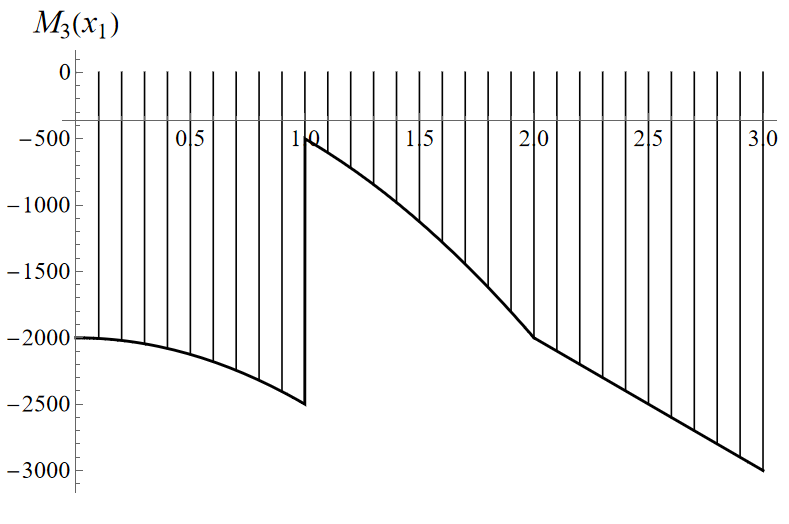
\includegraphics[width=0.7\linewidth]{plot-8}
		\caption{Эпюра изгибающего момента без учёта реакции $R_3$}
	\end{figure} 
	
	\begin{figure}[!h]
		\centering
		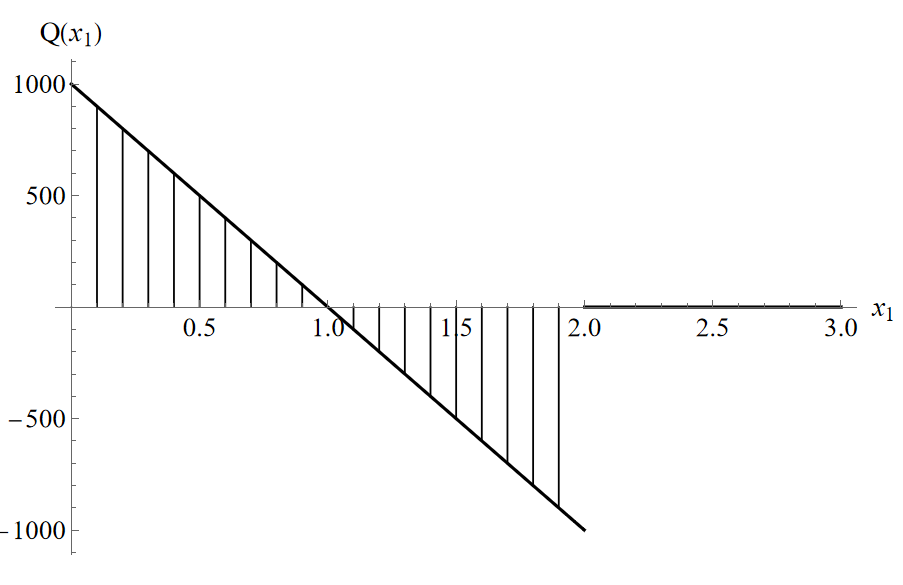
\includegraphics[width=0.7\linewidth]{plot-9}
		\caption{Эпюра перерезывающей силы без учёта реакции $R_3$}
	\end{figure}
	
	\vspace{-0.75em}
	
	\section{Прогиб статически определимой балки без $R_3$} 
	
	С учётом \eqref{eqw}, \eqref{eqwGU} и \eqref{eqM3NOR} прогиб статически определимой балки без реакции $R_3$
	\begin{equation}
		\begin{split}
			w(x_1) = \dfrac{1}{E J_3} \bigg[ M_1 f_2(x_1 - L) - M_0 & f_2(x_1) + P_1 f_3(x_1 - L) + P_2 f_3(x_1 - 2L) - \\ - q^{\circ} f_4(x_1) + q^{\circ} f_4(x_1 - 2L) + \dfrac{L^2}{24} \big( & 32 M_1 - 56 M_0 - 12L P_2 - 13L^2 q^{\circ} \big) + \\ & + \dfrac{L}{24} \big( 80 M_0 - 32 M_1 + 12L P_2 + 15 L^2 q^{\circ} \big) x_1 \bigg].
		\end{split}
		\label{eqwNOR} 
	\end{equation}
	
	В точке $x_1 = 3L$
	\vspace{-0.5em}
	\begin{equation}
		w_{0} = w(3L) = \dfrac{L^2}{24 E J_3} \left( -24 M_0 - 2 L^2 q^{\circ} \right).
		\label{eqw0}
	\end{equation}
	
	\newpage
	
	\section{Определение силы реакции $R_3$} 
	
	Для статически неопределимой балки в точке $x_1 = 0$ имеем закрепление, поэтому  прогиб в этой точке отсутствует. Тогда для определения силы реакции $R_3$ можно воспользоваться условием 
	\[
	w_{R_3} + w_0 = 0.
	\]
	
	С учётом \eqref{eqwR3} и \eqref{eqw0} имеем
	\begin{equation*}
		R_3 = \dfrac{L^2}{24 E J_3} \left( 24 M_0 +  2 L^2 q^{\circ} \right) \dfrac{3 E J_3}{L^3}.
	\end{equation*}
	
	Тогда из \eqref{eqP0P1} получим силы реакции для статически неопределимой балки
	\begin{equation*}
		\begin{cases}\vspace{0.75em}
			P_1 = \dfrac{51}{32} L q^{\circ} - \dfrac{7}{8} P_2 + \dfrac{1}{12L} (14 M_0 + M_2), \\
			P_0 = \dfrac{13}{96} L q^{\circ} - \dfrac{3}{8} P_2 + \dfrac{1}{12L} (M_0 + 2 M_1). \\
		\end{cases}
	\end{equation*}
	
	При значениях параметров в соответствии с индивидуальным заданием
	\vspace{-0.5em}
	\[
	R_3 = 6250 \; \text{Н}, \quad P_1 = -15750 \; \text{Н}, \quad P_0 = 10500 \; \text{Н}.
	\]
	
	\vspace{-1.5em}
	
	\section{Расчёт статически неопределимой балки}
	\subsection{Изгибающий момент и перерезывающая сила}
	
	Выражения для изгибающего момента и перерезывающей силы статически неопределимой балки можно получить путём сложения соответствующих выражений для балки под действием только силы реакции $R_3$, приложенной вместо отброшенной связи, а также статически определимой балки без учёта силы реакции $R_3$. 
	
	После сложения \eqref{eqM3QR} с \eqref{eqM3NOR} и \eqref{eqQNOR} соответственно c учётом \eqref{eqP0P1NOR} получим
	\vspace{-0.25em}
	\begin{equation*}
		\begin{split}
			M_3(x_1) = M_1 f_0(x_1 - L) - M_0 f_0(x_1) & + R_3 f_1(x_1) + \left( P_1 - \dfrac{3}{2} R_3 \right) f_1(x_1 - L) + \\ & + P_2 f_1(x_1 - 2L) - q^{\circ} f_2(x_1) + q^{\circ} f_2(x_1 - 2L).
		\end{split}
	\end{equation*}
	
	\vspace{-0.25em}
	
	С учётом \eqref{eqQ} перерезывающая сила
	\vspace{-0.25em}
	\begin{equation*}
		Q(x_1) =  R_3 f_0(x_1) + \left( P_1 - \dfrac{3}{2} R_3 \right) f_0(x_1 - L) - P_2 f_0(x_1 - 2L) - q^{\circ} f_1(x_1) + q^{\circ} f_2(x_1 - 2L). \\
	\end{equation*}
	
	Построим эпюры полученных изгибающего момента и перерезывающей силы для статически неопределимой балки при значениях параметров в соответствии с индивидуальным заданием.
	
	\newpage
	
	\begin{figure}[!h]
		\centering
		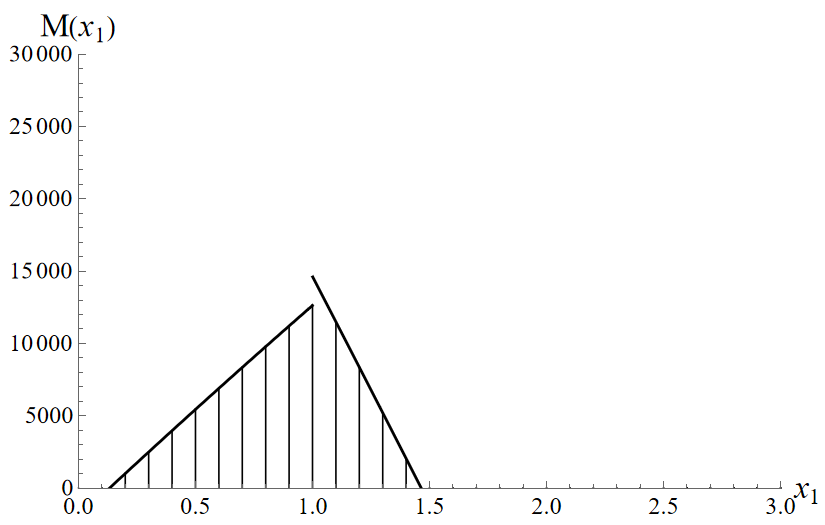
\includegraphics[width=0.75\linewidth]{plot-10}
		\caption{Эпюра изгибающего момента статически неопределимой балки}
	\end{figure} 
	
	\begin{figure}[!h]
		\centering
		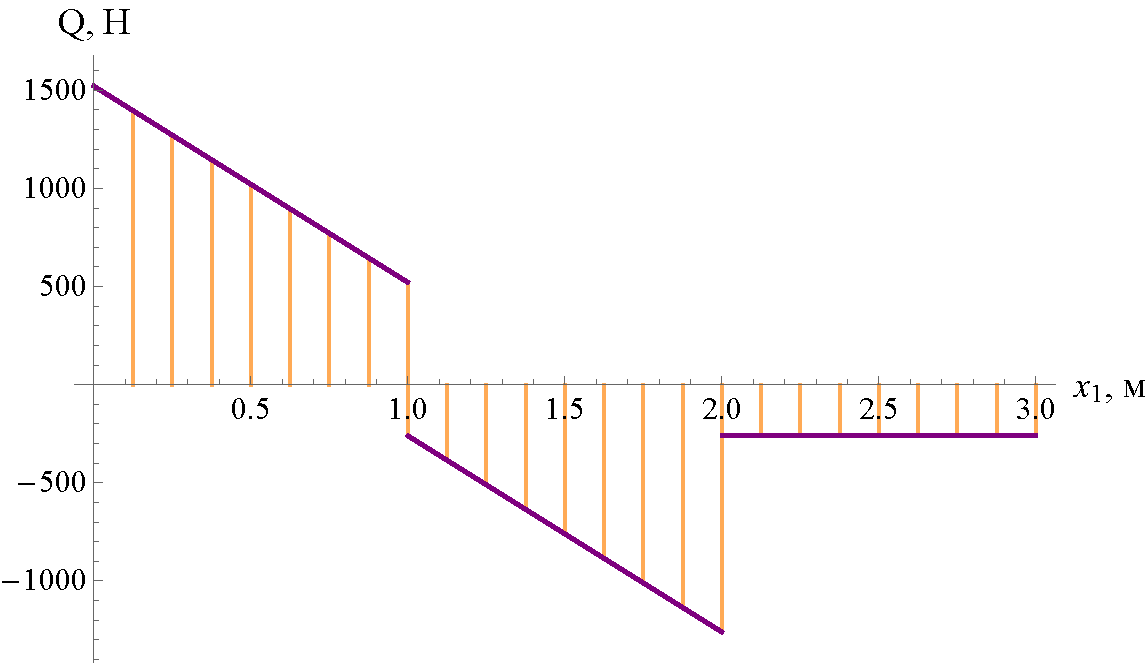
\includegraphics[width=0.75\linewidth]{plot-11}
		\caption{Эпюра перерезывающей силы статически неопределимой балки}
	\end{figure}
	
	\subsection{Прогиб исходной балки}
	
	Выражения для прогиба статически неопределимой балки также можно получить путём сложения соответствующих выражений для балки под действием только силы реакции $R_3$, а также статически определимой балки без учёта силы реакции $R_3$. 
	
	После сложения \eqref{eqwR} и \eqref{eqw0} c учётом \eqref{eqP0P1NOR} получим
	\vspace{-0.25em}
	\begin{equation*}
		\begin{split}
			w(x_1) = \dfrac{1}{E J_3} \bigg[ M_1 f_2(x_1 - L) - M_0 f_2(x_1) + R_3 & f_3(x_1) + \left( P_1 - \dfrac{3}{2} R_3 \right) f_3(x_1 - L) + \\ + P_2 f_3(x_1 - 2L) - q^{\circ} f_4(x_1) + q^{\circ} f_4(x_1 - 2L) & + \dfrac{L^2}{48} \big( 32 M_1 - 56 M_0 - 12L P_2 - 13L^2 q^{\circ} \big) + \\ & + \dfrac{L}{48} \big( 80 M_0 - 32 M_1 + 12L P_2 + 15 L^2 q^{\circ} \big) x_1 \bigg].
		\end{split}
	\end{equation*}
	
	\newpage
	
	Для балки с прямоугольным поперечным сечением с основанием $b$ и высотой $h$ осевой момент инерции относительно нейтральной оси имеет вид
	\[
	J_3 = \dfrac{b h^3}{12}.
	\]
	
	Построим график зависимости прогиба для статически неопределимой балки при значениях параметров в соответствии с индивидуальным заданием.
	
	\begin{figure}[!h]
		\centering
		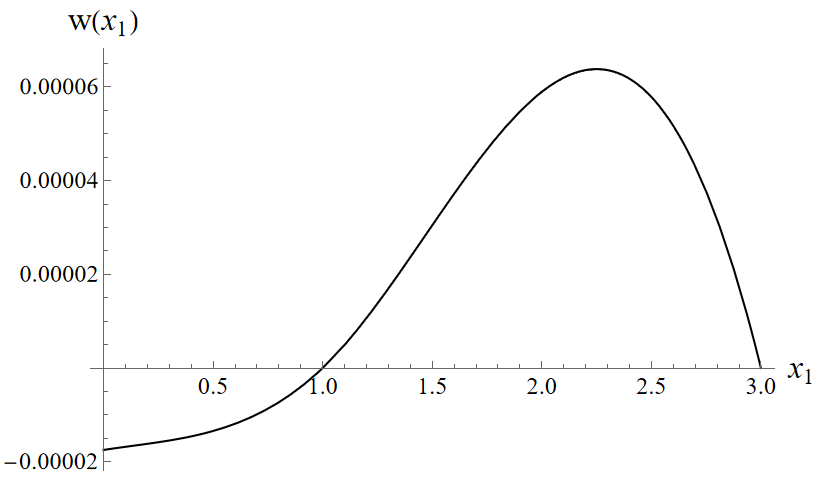
\includegraphics[width=0.75\linewidth]{plot-12}
		\caption{Прогиб статически неопределимой балки}
	\end{figure}
	
	\section{Наибольшее растягивающее напряжение}
	
	Максимальное растягивающее напряжение в поперечном сечении, симметричном относительно нейтральной оси, можно определить по формуле
	\[
	\sigma_{11}^{max} = \frac{M_3}{W_3}.
	\]
	
	Для прямоугольного поперечного сечения момент сопротивления сечения при изгибе имеет вид
	\[
	W_3 = \frac{b h^2}{6}.
	\]
	
	Наибольшее по абсолютной величине значение изгибающего момента $M_0$ достигается при $x_1 = 0$. Тогда 
	\[
	\sigma_{11}^{max} = 6 \frac{|M_0|}{b h^2}.
	\]
	
	При значениях параметров в соответствии с индивидуальным заданием
	\[
	\sigma_{11}^{max} \approx 94{,}675 \ \text{МПа}.
	\]
	
	\newpage
	\section{Заключение}
	
	В данной работе для заданной пары металлов были получены следующие результаты:
	\begin{enumerate}
		\item изображена схема нагружения статически неопределимой балки в соответствии с индивидуальным заданием;
		
		\item проверена степень статической неопределимости балки;
		
		\item в соответствии с индивидуальным вариантом осуществлён переход к статически определимой балке путём отбрасывания указанной в задании наложенной связи $P_0$ и замены её соответствующей реакцией $R_3$; 
		
		\item построены эпюры изгибающего момента и перерезывающей силы только от действия указанной выше реакции, приложенной вместо отброшенной связи (шарнирной опоры);
		
		\item найдена однозначная аналитическая зависимость величины прогиба балки под действием только реакции $R_3$;
		
		\item построены эпюры изгибающего момента и перерезывающей силы для статически определимой балки без учёта отброшенной связи и её силы реакции;
		
		\item для статически определимой балки найдена аналитическая зависимость величины прогиба от продольной координаты;
		
		\item из равенства нулю алгебраической суммы полученных в пп. 5 и 7 прогибов балки в сечении, соответствующем отброшенной опоре, получена зависимость реакции $R_3$ в этом сечении от остальных заданных параметров;
		
		\item для исходной статически неопределимой балки построены эпюры изгибающего момента и перерезывающей силы, а также определена зависимость прогиба балки от продольной координаты и построен график этой зависимости;
		
		\item для поперечного сечения балки с наибольшим по абсолютному значению изгибающим моментом найдено наибольшее растягивающее напряжение.
		
	\end{enumerate}
	
	\newpage
	\begin{thebibliography}{2}
		\bibitem{first-zarubin} Зарубин В.С., Кувыркин Г.Н. Математические модели механики и электродинамики сплошной среды. М.: Изд-во МГТУ им. Н.Э. Баумана, 2008. 512 с.
		\bibitem{second-zarubin} Зарубин В.\,С., Кувыркин Г.\,Н., Станкевич И.\,В. Математические модели прикладной механики. М.: Изд-во МГТУ им Н.\,Э. Баумана, 2016. 282 с.
		\bibitem{third-zarubin} Феодосьев В.\,И. Сопротивление материалов. 15-е изд. М.: Изд-во МГТУ им Н.\,Э. Баумана, 2010. 590 с.
	\end{thebibliography}
	
\end{document} 